
%% conf_paper.tex

\documentclass[conference]{IEEEtran}
% Add the compsoc option for Computer Society conferences.
%
% If IEEEtran.cls has not been installed into the LaTeX system files,
% manually specify the path to it like:
% \documentclass[conference]{../sty/IEEEtran}


% *** GRAPHICS RELATED PACKAGES ***
%
\ifCLASSINFOpdf
   \usepackage[pdftex]{graphicx}
  % declare the path(s) where your graphic files are
   \graphicspath{{../pdf/}{../jpeg/}}
  % and their extensions so you won't have to specify these with
  % every instance of \includegraphics
   \DeclareGraphicsExtensions{.pdf,.jpeg,.png}
\else
  % or other class option (dvipsone, dvipdf, if not using dvips). graphicx
  % will default to the driver specified in the system graphics.cfg if no
  % driver is specified.
   \usepackage[dvips]{graphicx}
  % declare the path(s) where your graphic files are
   \graphicspath{{../eps/}}
  % and their extensions so you won't have to specify these with
  % every instance of \includegraphics
   \DeclareGraphicsExtensions{.eps}
\fi

%=========================================================
% Latex Packages
%=========================================================
\usepackage{listings}
\usepackage{xspace}
\usepackage[colorlinks=true,linkcolor=blue,citecolor=blue,urlcolor=blue]{hyperref}
\usepackage[colorinlistoftodos,textwidth=2.5cm,shadow]{todonotes}

%=========================================================
% Other
%=========================================================

\usepackage{color}
\usepackage{listings}


%\newcommand{\comment}[1]{\textcolor{red}{#1}}
\definecolor{keywordcolor}{rgb}{0.5,0,0.33}
\definecolor{identifiercolor}{rgb}{0,0,0.75}
%\definecolor{commentcolor}{rgb}{0.25,0.5,0.37}
\definecolor{commentcolor}{rgb}{0.3,0.3,0.3} 

\lstdefinelanguage{bon} {
  morekeywords={class_chart,indexing,explanation,part,query,command,constraint,
  end,deferred,effective,persistent,require,ensure,invariant,feature,class,
  static_diagram,component,old,not,inherit,delta,for_all,such_that,it_holds,Current,Lockset,when,monitors_for,max,concurrency,concurrent,guarded,locks,special,failure,sequential,atomic},
  morekeywords={[2]LOCK,SEMAPHORE,BOOLEAN,INTEGER,REAL,SEQUENCE,MAIN,EXCEPTION,NO_SEATS,BARBER_SHOP,CUSTOMER,BARBER},
  morekeywords={[3]},
  morecomment=[l]{--}, morestring=[b]", morestring=[d]'
  }[keywords,comments,strings]

\lstdefinestyle{bon}{language={bon},showstringspaces={false},
  basicstyle={\scriptsize\ttfamily\mdseries},
  keywordstyle={\color{keywordcolor}},
  keywordstyle={[2]\color{black}\bfseries},
  keywordstyle={[3]\color{black}\bfseries},
  identifierstyle={\color{identifiercolor}},
  commentstyle={\color{commentcolor}},
  frame=lines}

\lstdefinestyle{boninline}{language={bon},showstringspaces={false},
  basicstyle={\ttfamily\mdseries},
  keywordstyle={\color{black}},
  keywordstyle={[2]\color{black}\bfseries},
  keywordstyle={[3]\color{black}\bfseries},
  identifierstyle={\color{black}\mdseries},
  commentstyle={\color{black}},
  frame=lines,
  columns=fullflexible,
  breaklines=true}
\lstset{style=bon, columns=fullflexible, keepspaces=true, 
        frame=topline, captionpos=b}

%=========================================================
% Generic Macros
%=========================================================

\newcommand{\lstbon}[1]{\lstinline[style=boninline]{#1}} 
\newcommand{\lstjava}[1]{\lstinline[style=jml2inline]{#1}} 

\newcommand{\eg}{e.g.,\xspace}
\newcommand{\ie}{i.e.,\xspace}
\newcommand{\etc}{etc.\xspace}
\newcommand{\vs}{vs.\xspace}
\newcommand{\etal}{et.~al.\xspace}

% Todos
\newcommand{\note}[1]{\todo[inline,color=red!40]{#1}}

% correct bad hyphenation here
\hyphenation{op-tical net-works semi-conduc-tor}

% =========================================================

\begin{document}
%
% paper title
% can use linebreaks \\ within to get better formatting as desired
\title{A Rigorous Methodology for Analyzing and Designing Plug-ins}


% author names and affiliations
% use a multiple column layout for up to three different
% affiliations
\author{
\IEEEauthorblockN{ Marieta V. Fasie}
\IEEEauthorblockA{DTU Compute\\Technical University of Denmark\\
DK-2800 Lyngby, Denmark\\
Email: marietafasie@gmail.com}

\and

\IEEEauthorblockN{ Anne E. Haxthausen}
\IEEEauthorblockA{DTU Compute\\Technical University of Denmark\\
DK-2800 Lyngby, Denmark\\
Email: ah@imm.dtu.dk}

\and

\IEEEauthorblockN{Joseph Kiniry}
\IEEEauthorblockA{DTU Compute\\Technical University of Denmark\\
DK-2800 Lyngby, Denmark\\
Email: jkin@imm.dtu.dk}}

% use for special paper notices
%\IEEEspecialpapernotice{(Invited Paper)}


% make the title area
\maketitle

% =========================================================
% Abstract
% =========================================================

\begin{abstract}
%\boldmath
  Today, GUI plug-ins development is typically done in a very ad-hoc
  way, where developers dive directly into implementation.  Without
  any prior analysis and design, plug-ins are often flaky, unreliable,
  difficult to maintain and extend with new functionality, and have
  inconsistent user interfaces.  This paper addresses these problems
  by describing a rigorous methodology for analyzing and designing
  plug-ins.  The methodology is grounded in the Extended Business
  Object Notation (EBON) and covers informal analysis and design of
  features, GUI, actions, and scenarios, formal architecture design,
  including behavioral semantics, and validation.  The methodology is
  illustrated via a case study whose focus is an Eclipse environment
  for the RAISE formal method's tool suite.
\end{abstract}

% no keywords

% For peer review papers, you can put extra information on the cover
% page as needed:
% \ifCLASSOPTIONpeerreview
% \begin{center} \bfseries EDICS Category: 3-BBND \end{center}
% \fi
%
% For peerreview papers, this IEEEtran command inserts a page break and
% creates the second title. It will be ignored for other modes.
\IEEEpeerreviewmaketitle


% =========================================================
% Introduction
% =========================================================
\section{Introduction}
\label{sec:introduction}

What is the paper about.

% Background
%
\subsection{Background}
\label{sec:background}

What problems do we run into when starting building an Eclipse plug-in.

About the case study:  RAISE method~\cite{RMG95},
RAISE Specification Language~\cite{RLG92} 
% Related work
%
\subsection{Related work}
\label{sec:related-work}

What solutions have other papers brought

% =========================================================
% Analysis and design method
% =========================================================
\section{Analysis and design method}
\label{sec:analys-design-meth}

This section describes a methodology used to analyze and design
plug-ins. The methodology has six stages, each described in a separate
subsection and presented in the order in which they are applied. These
six steps are: \emph{domain modeling}, \emph{user interface},
\emph{events}, \emph{components}, \emph{components communication} and
\emph{code generation}.

The methodology is illustrated on a case study taken from a real
project in which an Eclipse environment for the RAISE formal method's
tool suite is being developed. Due to space restrictions, the entire
project's analysis and design phases are not presented here; instead,
only one scenario of the plug-in is shown from beginning to end.

% Domain Modeling
%
\subsection{Domain Modeling}
\label{sec:domain-modeling}

The first step when analyzing and designing a system is to establish
its domain model. This is done in order to create a common vocabulary
between those involved in the project and to identify the concepts
used in the product development process. This means that the most
important entities and terminology related to the system domain must
be identified, explained documented from the very beginning so they
can be unanimous understood and used throughout the entire product
life cycle.

\note{-Should we write that is "at a very high level" and "also meant
for non technical people"? Because in our case we are a little
technical -Also where do we describe the case study? -mvf}

Looking at the case study name and description, the domain model is
constructed by analyzing areas like Eclipse, RAISE and graphical user
interface (GUI). The result is a list of terminologies along with
their explanation, essentially describing entities and elements from a
high level point of view. Some examples from the list are notions
like \emph{editor, console, typechecker, translator, SML translator,
\LaTeX\ generator, SML compiler, RSL Perspective} and so on. Some of
these items can be grouped in a bigger entity, while others are
big enough to covers multiple notions. For example \emph{SML translator}
and \emph{\LaTeX\ generator} can be grouped under the
\emph{translator} notion, since both are referring to the process of
transforming a RSL specification into another type of specification.
Likewise \emph{RSL Perspective} can be seen as a notion that comprises
all other items since inside Eclipse all RAISE elements can be grouped
under a single perspective.

\lstset{style={bon}}
\lstinputlisting[style=bon, float=tp,label={example:system_chart},
caption={System chart describing the RAISE system.},
captionpos=b]{system_chart_example.bon}

All those described before can easily be captured in EBON using
\emph{system\_chart}, \emph{cluster\_chart} and \emph{class\_chart}
elements. The notions that have been identified are documented as
classes, which can be grouped under clusters and all these are
composing a big and unique system. \autoref{example:system_chart}
illustrates a caption of the RAISE System.

% User Interface
%
\subsection{User interface}
\label{sec:user-interface}

The purpose of this step is to determine the plug-in functionality from the
user's point of view. This means identifying all the things a user can
do from the plugin's user interface (UI). This UI feature set
consequently derives the requirements for the product (the plugin) and
designs the UI in the same time. Therefore, for each user action that
is relevant and important for the plug-in, a mock-up user interface is
created. If many user actions are similar, they can be grouped under a
single user interface. It is up to the plug-in developer to determine
what are the most important features and how, or if, she wants to
prioritize them.

The mock-up user interface can be a vague handmade sketch or a
precise drawing made with an advanced graphical editing program.  The
intention here is not presentation and precision, but instead feature
completeness and UI consistency.

For the Eclipse case study, it was decided, for example, that a user
should have the possibility to typecheck all RAISE Specification
Language (RSL) files (the primary file type of the RAISE tool suite).
Also, the user should have the possibility to translate all files to
SML, to run all test cases existing in all files, and to generate
\LaTeX\ documents for them.  Therefore, it was decided that these four
actions should be grouped under a menu item which is called \emph{RSL}
and presented in the same UI, for consistency and simplicity.  

\begin{figure}[!t] \centering
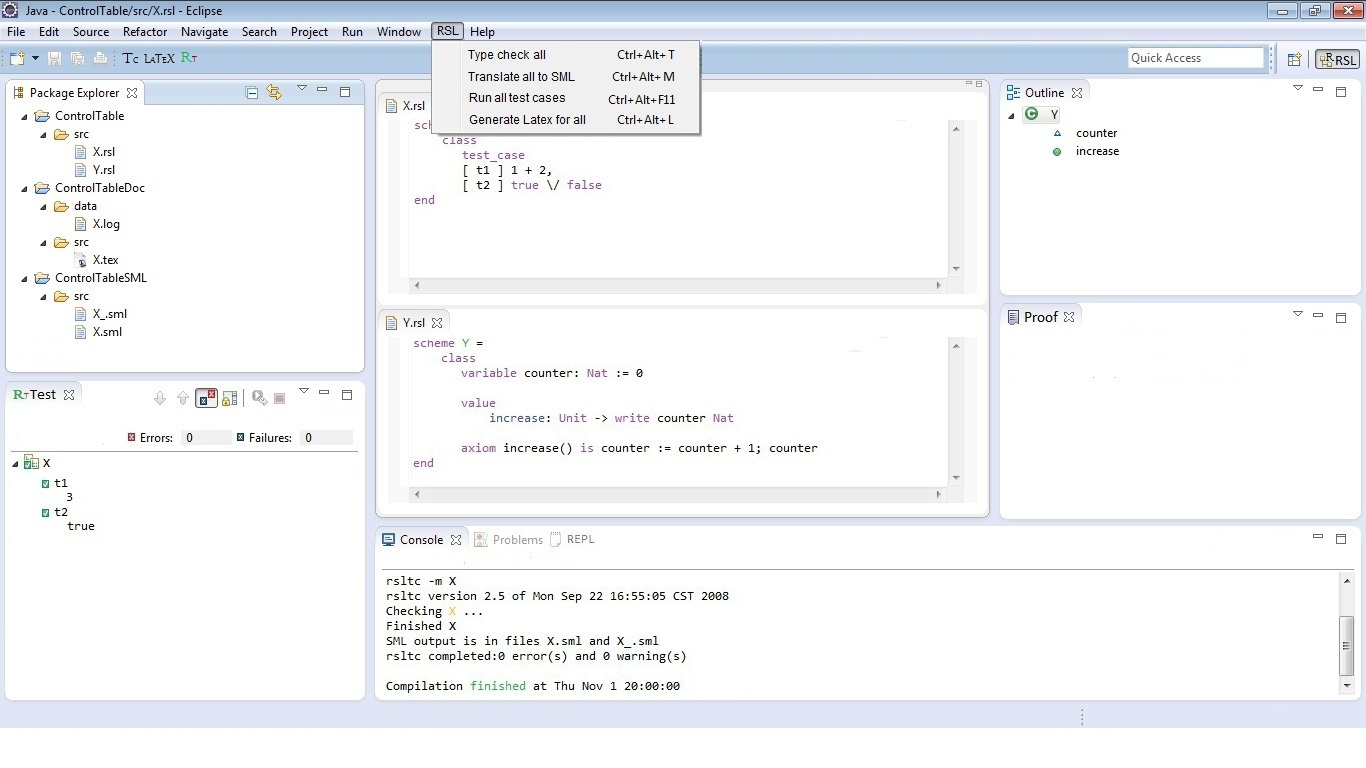
\includegraphics[width=2.5in]{RSLMenu.jpeg} 
% where an .eps filename suffix will be assumed under latex, 
% and a .pdf suffix will be assumed for pdflatex; or what has
% been declared via \DeclareGraphicsExtensions. 
\caption{Eclipse user interface displaying the RSL menu item} 
\label{UIMenu} 
\end{figure}

\note{These figures will have to span both columns to be viewable, I
  suspect. -jrk}

\autoref{UIMenu} illustrates the graphical user interface for the
\emph{RSL} menu item.  This illustration was created by taking a
screenshot of Eclipse and then hand-editing the resulting image in
just a few minutes.

\lstset{style={bon}}
\lstinputlisting[style=bon, float=tp,label={example:scenario_chart},
caption={Scenario chart for RSL menu.},
captionpos=b]{scenario_example.bon}

While the user interface is being drawn, product requirements are
documented using EBON \emph{scenario\_chart} elements.  The beautiful
part about using EBON from the beginning is that it allows the
requirements specification to be captured using natural language.
Therefore no intermediate step is required between identifying the
requirements and documenting them.  
For the case study, the requirements associated with the user
interface in \autoref{UIMenu} are captured in the
\emph{scenario\_charts} in \autoref{example:scenario_chart}.

% Events
%
\subsection{Events}
\label{sec:events}

In this section the entire system is seen as a black box. The focus is
on the external actions that make the system react and on the system
outgoing responses. However, not all systems outgoing events are of
interest, but only the ones that are started by external stimuli. 

An incoming external event is any action that determines the system to
change its state. For example it can be a user clicking a button or
another system sending a request. An outgoing internal event is the
response the system sends to the one that initiated the incoming
external event. The system outgoing event for the action of pressing
the button could e.g. be the display of a new window or writing a
message to the standard output.

Looking back at the scenario presented in
\autoref{sec:user-interface}, the user has the possibility to type
check all RSL files. This is illustrated in \autoref{UIMenu} by the
presence of a sub-menu item named \emph{Type check all}. Therefore,
the incoming external action in this case is: \emph{the user selects
the Type check all sub-menu item}. And this external event has been determined
just by looking at the scenarios previously identified. However there
is another user event that triggers the same system reaction and that
is using the shortcuts: \emph{The user presses Ctrl+Alt+T}.

\lstset{style={bon}}
\lstinputlisting[style=bon, float=tp,label={example:event_chart},
caption={Incoming event chart for typechecking features.},
captionpos=b]{external_event_example.bon}

Once established, the user actions can be captured in EBON using
\emph{event\_chart} elements. The \emph{event\_chart} can be ingoing
or outgoing based on which events they capture. Since the two user
incoming events that have just been identified aims for the same
functionality, they are grouped under the same name and captured in
\autoref{example:event_chart}.

\lstset{style={bon}}
\lstinputlisting[style=bon, float=tp,label={example:event_chart_in},
caption={Outgoing event chart for typechecking features.},
captionpos=b]{internal_event_example.bon}


All incoming actions trigger changes in the system state. And the
next task is to decide how should the system notify the one triggering the
action, about the changes that have taken place. For the RAISE case
study it was decided that after the user selects the \emph{Type check
all} sub-menu item, a message should be displayed on the standard output.
The message informs the user about how the typechecking evolved and
since the case study GUI is Eclipse based, the standard output is considered by
default the Eclipse Console view. However in some cases the
typechecking may not be successful due to some errors in the input
files. In this case it would be nice to know what caused the problem
and where can it be found. Therefore the system will present the
necessary information in the Eclipse Problem view. To sum up, after the
user selects the \emph{Type check all} sub-menu item, the system updates the
Console and Problem views with appropriate information.
\autoref{example:event_chart_in} presents the two events captured in
an outgoing \emph{event\_chart} under the names of
\emph{CONSOLEUPDATE} respectively \emph{PROBLEMSUPDATE}.


% Components
%
\subsection{Components}
\label{sec:components}

Major components captured in BON \emph{static\_diagram}s obtained from
\emph{cluster\_chart}, \emph{cluster\_chart} and \emph{class\_chart}.

-High level classifiers into concrete data types in language
independent fashion.

-"fully typed class interfaces and formal specification of software contracts"

% Components communication
%
\subsection{Components communication}
\label{sec:comp-comm}

How components are arranged.

Component interfaces added to the interface diagram using
\emph{feature}, \emph{require} and \emph{ensure}. This will later
result in plug-in extensions and extension points.

Update scenarios with events.

% Code generation
%
\subsection{Code generation}
\label{sec:code-generation}

Beetlz generates the Java code from BON specification.

% =========================================================
% Conclusion
% =========================================================
\section{Conclusion}
\label{sec:conclusion}

In conclusion

% conference papers do not normally have an appendix

% use section* for acknowledgement
\section*{Acknowledgment}
\label{sec:acknowledgment}

The authors would like to thank themselves by buying tons of chocolate
and beer. They really deserve it. 

% trigger a \newpage just before the given reference
% number - used to balance the columns on the last page
% adjust value as needed - may need to be readjusted if
% the document is modified later
%\IEEEtriggeratref{8}
% The "triggered" command can be changed if desired:
%\IEEEtriggercmd{\enlargethispage{-5in}}

% references section

% can use a bibliography generated by BibTeX as a .bbl file
% BibTeX documentation can be easily obtained at:
% http://www.ctan.org/tex-archive/biblio/bibtex/contrib/doc/
% The IEEEtran BibTeX style support page is at:
% http://www.michaelshell.org/tex/ieeetran/bibtex/
%\bibliographystyle{IEEEtran}
% argument is your BibTeX string definitions and bibliography database(s)
%\bibliography{IEEEabrv,../bib/paper}
%
% <OR> manually copy in the resultant .bbl file
% set second argument of \begin to the number of references
% (used to reserve space for the reference number labels box)
%
\bibliographystyle{IEEEtran}
\bibliography{main-bib}
%\begin{thebibliography}{1}

%\bibitem{IEEEhowto:kopka}
%H.~Kopka and P.~W. Daly, \emph{A Guide to \LaTeX}, 3rd~ed.\hskip 1em plus
% 0.5em minus 0.4em\relax Harlow, England: Addison-Wesley, 1999.

%\end{thebibliography}

% that's all folks
\end{document}


